\section{Background}

%%In order to calculate the shutdown dose rate of a nuclear systems,
%%a nuclear inventory must be calculated

\subsection{Nuclear Inventory Analysis}
When a material is irradiated a variety of reactions can happen. These 
reactions may lead to production of radionuclides which can persist
after shutdown of the device. For Shutdown Dose Rate (SDR) Analysis, 
the nuclear inventory must be known
in order to quantify the photon emission density as a function of time.
The rate at which a nuclide $i$ undergoes a reaction or decay to some 
other nuclide $j$ is given by Equation \ref{total_p_const}.

\begin{equation}\label{total_p_const}
  P_{i \rightarrow j, total} = P_{i \rightarrow j, reaction } +
  P_{i \rightarrow j, decay}
\end{equation}
The reaction process is described by Equation \ref{reaction_p_const}
\begin{equation}\label{reaction_p_const}
  P_{i \rightarrow j, reaction } =
  \int_{E_{n}} \sigma_{i \rightarrow j}(E_{n})
  \phi_{n}dE_{n}
\end{equation}
where $\sigma_{i \rightarrow j}(E_{n})$ is the microscopic cross
section for the reaction that transforms nuclide $i$ into $j$, and
 $\phi_{n}(E_{n})$ is the neutron flux for energy $E_{n}$.
The decay process is described by Equation
\ref{decay_p_const}

\begin{equation}\label{decay_p_const}
  P_{i \rightarrow j, decay} = \lambda_{i} b_{i \rightarrow j}
\end{equation}
where $\lambda_{i}$ is the decay constant and $b_{i \rightarrow j}$ is
the branching ratio.
The rate of change in the concentration of nuclide $i$ is given by the 
difference of production and destruction of that nuclide. 
\begin{equation}\label{rate_change_i}
  \frac{dN_{i}(t)}{dt} = \sum_{j} N_{j}P_{j \rightarrow i, total}
  - \sum_{j} N_{i}P_{i \rightarrow j, total}
\end{equation}

This can be expressed as a system of differential equations for an 
entire network of nuclides. 
\begin{equation}
  \frac{dN}{}
\end{equation}

\subsection{Shutdown Dose Rate Workflow}

A primary method to investigate the shutdown dose rate is known as the
Rigorous 2-Step (R2S) method. The R2S method consists of two transport steps
coupled by an activation step. 
A neutron transport is first performed, and the neutron flux tallied.
The neutron fluxes, and an irradiation scenerio are used in an activation
calculation using a dedicated nuclear iventory analysis code to give the 
photon density in the region as function of time. 
This photon density is then used as a source for photon transport,
where the SDR is tallied using a tally modified with flux-to-dose-rate
conversion factors.


% \begin{figure}[h!]
% \begin{centering}
% 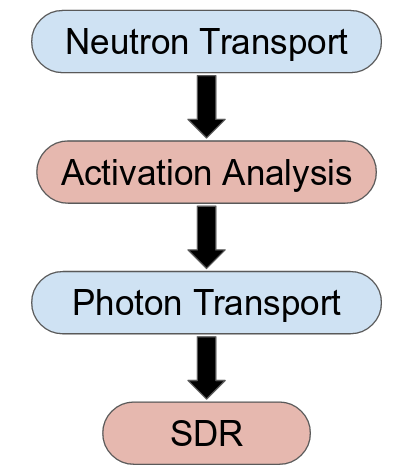
\includegraphics[scale=0.3]{../figs/r2s.png}
% % \frame{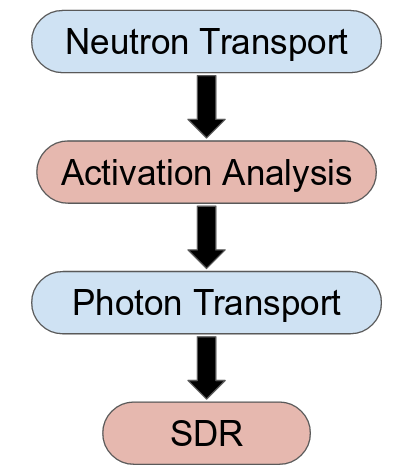
\includegraphics[width=0.30\linewidth, height=4cm]{../figs/r2s.png}}
% \caption{General shutdown dose rate workflow}
% \label{r2s}
% \end{centering}
% \end{figure}

\subsection{Shutdown Dose Rate for High Energy Systems}
One of the challeges presented when analyzing high energy systems is the 
lack of nuclear tables in the energy range higher than 20 MeV. 
As seen in Equation \ref{raction_p_const}, the flux has to be folded 
with reaction cross sections to obtain production and destruction rates.
To gap this bridge, some activation codes accept productions and destruction rates
as their input.
% This has previously been done by pos-processing high energy files from the 
% neutron transport to obtain Production and Destruction cross sections.




The current SDR workflow is seen in Figure \ref{rnucs_r2s}
\begin{figure}[ht!]
\begin{centering}
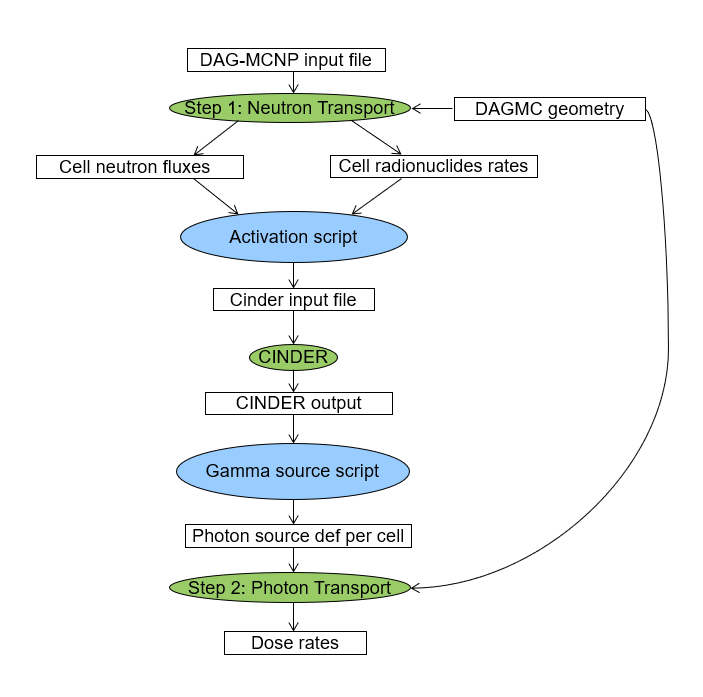
\includegraphics[scale=0.4]{../figs/rnucs_r2s.png}
\caption{Current shut down dose rate workflow for Accelerator systems as used by ORNL}
\label{rnucs_r2s}
\end{centering}
\end{figure}
